
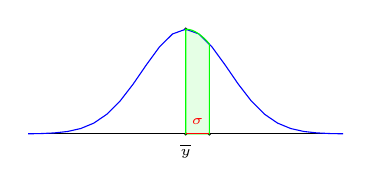
\begin{tikzpicture}
\draw (-2.,0) -- (2,0);
\draw[fill] (0,0) circle [radius=0.0125];
\node [below] at (0,0) {\tiny $\overline{y}$};

\draw[fill] (0.3,0) circle [radius=0.0125];
\draw[fill] (0,1.33) circle [radius=0.0125];
\draw (0,0) -- (0,1.33);


\draw[blue, domain=-2:2,] plot (\x, {1/(0.3*sqrt(2*pi))*exp(-(\x*\x)/(2*0.3))});
\draw[green, domain=-0:0.3,fill,fill opacity=0.1] (0,0) -- plot (\x, {1/(0.3*sqrt(2*pi))*exp(-(\x*\x)/(2*0.3))}) -- (0.3,0) -- cycle;

\node [above,red] at (0.15,0) {\tiny $\sigma$};
\draw [red](0.,0) -- (0.3,0);
\end{tikzpicture}